\chapter{The numerical model EULAG}

Refer to work of Grogger that investigated deep propagating GWs, individual spectral forcings, linear analysis vs numerical results...

Grogger also showed EULAG simulations for transient lower boundary, more specifically growing amplitude / rising topography 

extend with the comparing numerical to analytical results of GWD for different MW regimes...
and show transient lower boundary moving in x-direction

\section{General setup}
\label{sec:EULAG}

The nonlinear numerical simulations are conducted with the EUlerian/semi- LAGrangian fluid solver (EULAG). The model is set up solving the soundproof anelastic set of equations (\cite{lipps_scale_1982}) consisting of the three components of the momentum equation (\ref{equ:momEqu}), the thermodynamic equation (\ref{equ:potTemp}) for the potential temperature perturbation $\theta$'=$\theta-\theta_e$ and the mass continuity equation (\ref{equ:continuityEqu}):
%
\begin{equation}
\begin{aligned}
    \frac{d \Vec{v}}{dt} = -G \Vec{\nabla} (\frac{p'}{\bar{\rho}}) +  \Vec{g} \frac{\theta'}{\bar{\theta}} - 2 \Vec{\Omega} \times (\Vec{v}-\Vec{v_e}) \\
    - \Tilde{\alpha} (\Vec{v}-\Vec{v_e}) \equiv R^{v},
    \label{equ:momEqu}
\end{aligned}
\end{equation}
%
\begin{equation}
    \frac{d \theta'}{dt} = -\Vec{v} \cdot \Vec{\nabla} \theta_e - \Tilde{\beta} (\theta-\theta_e) \equiv R^{\theta},
    \label{equ:potTemp}
\end{equation}
%
\begin{equation}
    \Vec{\nabla} \cdot (\bar{\rho} \Vec{v}) = 0.
    \label{equ:continuityEqu}
\end{equation}
%
Here, $\frac{d}{dt}$, $\Vec{\nabla}$ and $\Vec{\nabla} \cdot$ represent the total derivative, the gradient and the divergence respectively. $p'$ is the pressure perturbation with respect to the environmental state, g the gravitational acceleration and $\Vec{\Omega}$ the angular velocity of the Earth. The matrix G represents geometric terms, which result from the general, time-dependent coordinate transformation and the symbol $R^{\Psi}$ stands for the right-hand side of the corresponding equations for the variables $\Psi = (u,v,w,\theta')$.
%
\begin{equation}
    \bar{\theta}(z) = \theta_0 \textrm{ exp}(-\frac{N^2}{g} z) 
    \label{equ:thetaScale}
\end{equation}
%
and the anelastic density 
%
\begin{equation}
    \bar{\rho}(z) = \rho_0 \textrm{ exp}(-\frac{z}{H_{\rho}})
    \label{equ:densityScale}
\end{equation}
% with $H_{/rho} = 7314m$. 
refer to the hydrostatic reference state around a constant stability profile as introduced by \textcite{bacmeister_breakdown_1989} with stability $\frac{N^2}{g}$, a density scale height $H_{\rho}$ that corresponds to a deep atmosphere and $\rho_0$, $\theta_0$ set to appropriate reference constants. With (\ref{equ:thetaScale}) and (\ref{equ:densityScale}) being the basic state of equations (\ref{equ:momEqu}-\ref{equ:continuityEqu}), a more general environmental state, which reflects the initial and boundary conditions, enters the equations via the variables with subscript e. In that sense, $\alpha(\Vec{v}-\Vec{v_e})$ and $\beta(\theta-\theta_e)$ represent relaxation terms, which enable the radiation of wave energy across the model boundaries and force the solutions at the model boundaries to the prescribed environmental profiles. These ambient states like $u_e$, $\rho_e$ or $\theta_e$ can be time-dependent to replicate transient flow conditions, but are stationary within the scope of this thesis. On the other hand, transient boundaries like a propagating tropopause fold almost demand for time-dependent terrain-following vertical coordinates as introduced by \textcite{wedi_extending_2003}, so this option may be considered at a later stage. Furthermore, EULAG is noteworthy for its robust elliptic solver (\cite{smolarkiewicz_forward--time_1993}) and generalized coordinate formulation enabling grid adaptivity technology (\cite{prusa_eulag_2008}, \cite{kuhnlein_modelling_2012}).

As the name suggests, EULAG is capable of solving the equations of motion (\ref{equ:momEqu}-\ref{equ:continuityEqu}) in an Eulerian (flux form) or in a semi-Lagrangian (advective form) mode (\cite{smolarkiewicz_forward--time_1997}). For the numerical approximation it utilizes a non-oscillatory forward-in-time (NFT) approach compactly formulated as
%
\begin{equation}
\begin{aligned}
    \Psi^{n+1} = LE(\Tilde{\Psi}, V^{n+1}, G^n, G^{n+1}) \\
    + \frac{1}{2} \Delta t R^{\Psi} |^{n+1}
    \label{equ:NFTscheme}
\end{aligned}
\end{equation}
%
with $LE$ representing the corresponding semi-Lagrangian/Eulerian transport operator. The NFT scheme belongs to the class of second-order-accurate two-time-level algorithms that are build on nonlinear advection techniques (\cite{prusa_eulag_2008}). These schemes have the property to suppress and control numerical oscillations that are often found in higher order linear schemes. As a result, transporting the auxiliary field $\Tilde{\Psi} = \Psi^n + \frac{1}{2} \Delta t R^{\Psi}|^n$ instead of the specific variable $\Psi$, results from a thorough truncation error analysis and ensures second order accuracy. (\cite{smolarkiewicz_forward--time_1997}).

Within the scope of this Master's thesis all simulations utilize the Eulerian option by applying the multidimensional positive definite advection transport algorithm MPDATA (\cite{smolarkiewicz_mpdata_1998} and  and \cite{smolarkiewicz_multidimensional_2006}).

EULAG has a proven itself as a reliable tool for simulating thermo-fluid flows across the wide range from turbulent to global scales (\cite{prusa_all-scale_2003}) and in a variety of of physical scenarios like e.g. turbulence, GW dynamics, flows past complex/moving boundaries, micrometeorology or cloud microphysics (\cite{prusa_eulag_2008}). A comparison between different well-established numerical models (including EULAG) and their capability to model flow over steep terrain, which is relevant for the investigations within this thesis, appears in \textcite{doyle_intercomparison_2011}.

%%%%% NOTES %%%%%
% Prusa 2008 also has good description of perturbation form and points out importance of correct environmental/initial state!! 

% \cite{smolarkiewicz_multidimensional_2006}

% \begin{equation}
%    \frac{\partial G \rho \Psi}{\partial t} + \nabla \cdot G \rho \Vec{v} = G \rho R
%    \label{equ:statMeshAdapt}
% \end{equation}


% he elliptic pressure equation is solved via a preconditioned non-symmetric Krylov sub- space solver (Smolarkiewicz and Margolin; 1994; 1997, Skamarock et al., 1997).

% imlicit /explicit elliptic pressure solver / krylov sub space solver

% There, governing equations are formulated in general- ized time-dependent curvi-linear coordinates to enable mesh adaptivity (Prusa and Smolarkiewicz 2003; Wedi and Smolarkiewicz 2004; Kühnlein et al. 2012; Smolarkiewicz and Charbonneau 2013) and continuous mappings of the Earth’s topography by using terrain-following coordinates (Gal-Chen and Somerville 1975; Clark 1977)


% anelastic -> elastic energy is not allowed -> sound waves are filtered since they are based on pressure difference rather then temperature


\section{Ambient profiles of idealized simulations}
% mark variables to be defined in table!! like in isentropic paper lightcyan
profile of potential temperature (definition of N) sets up background profiles


choice of kappa is not relevant for simulations with using the soundproof anelastic equations similar to \textcite[]{lipps_scale_1982}. The correct value for diatomic gases is $\kappa=\frac{2}{7}$. For simulations of the stratosphere with N=0.02 This leads to a reasonable temperature of 239K, but for N=0.01, a reasonable value for the troposphere, ambient profiles following \textcite{bacmeister_breakdown_1989} would result in T=900k. Therefore, T = 290K... with K=


EULAG provides multiple options to define background states of the atmosphere. For the presented simulations vertical ambient profiles define an isothermal atmosphere with constant stability as described by \textcite{bacmeister_breakdown_1989}. These exponential profiles of potential temperature and density avoid physical restrictions towards higher altitudes and are thus well suited for the investigation of deep gravity wave propagation. Defining a potential temperature and density scale height $H_{\Theta}$ and $H_{\rho}$ leads to


\begin{equation}
    \bar{\theta}(z) = \theta_0 \textrm{ exp}(-\frac{N^2}{g} z) 
    \label{equ:thetaScale}
\end{equation}
%
and the anelastic density 
%
\begin{equation}
    \bar{\rho}(z) = \rho_0 \textrm{ exp}(-\frac{z}{H_{\rho}})
    \label{equ:densityScale}
\end{equation}
% with $H_{/rho} = 7314m$. 
refer to the hydrostatic reference state around a constant stability profile as introduced by \textcite{bacmeister_breakdown_1989} with stability $\frac{N^2}{g}$, a density scale height $H_{\rho}$ that corresponds to a deep atmosphere and $\rho_0$, $\theta_0$ set to appropriate reference constants.

\begin{equation}
\begin{aligned}
    p_0(z) &= p_{00} e^{-\frac{z}{H_{\rho}}} \quad \textrm{with} \quad H_{\rho} = \frac{R_d}{c_p} H_{\Theta} = \frac{R_d T_{00}}{g} \\
    \rho_0(z) &= \frac{p_0(z)}{R_d T_{00}} = \rho_{00} e^{-\frac{z}{H_{\rho}}} \\
    T_0(z) &= \frac{p_{00}}{R_d \rho_{00}} \\
    \Theta_0(z) &= T_{00} \frac{p_{00}}{p}^{\kappa} \\
    \Theta_0(z) &= T_{00} e^{\frac{z}{H_{\Theta}}} \quad \textrm{with} \quad H_{\Theta} = \frac{g}{N^2} \\
    \label{equ:ambient-Profiles}
\end{aligned}
\end{equation}
% based on hydrostatic approximation dp/dz = -rho*g -> pressure with density scale height

with the Brunt-Vaisala frequency $N$, the specific gas constant $R_d$ and the specific heat capacity at constant pressure $c_p$. $p_0$, $\rho_0$ and $T_0$ represent a reference state of the atmosphere.

\begin{table*}[ht]
\centering
\caption{Parameters related to the ambient reference state and vertical profiles following \textcite[]{bacmeister_breakdown_1989}. Values for the troposphere are used for the model validation in section \ref{sec:linear-MWs}. Values for the stratosphere are used for the main simulations of this thesis described in chapters \ref{sec:resultsQ3D} and \ref{sec:results3D}. Colored cells refer to parameters that need to be defined.}

%%%% include trop for diatomic gas - then explain difference
%%% do scaled values still make sense
\begin{tabular}{@{}cccc@{}}
\toprule
 & Unit & Troposphere & Stratosphere \\ \midrule[1pt]

$R$ & J kg$^{-1}$ K$^{-1}$ &   \cellcolor{LightCyan} 287.04 &   \cellcolor{LightCyan} 287.04 \\
$g$ & m s$^{-2}$ & \cellcolor{LightCyan} 9.80616 & \cellcolor{LightCyan} 9.80616 \\
$N$ & s$^{-1}$ & \cellcolor{LightCyan} 0.01 & \cellcolor{LightCyan} 0.02 \\
$H_{\Theta}$ & m & 98061.6 & 24515.4  \\
$H_{\rho}$ & m & 28017.6 (8011.3)  & 7004.4 \\
$\kappa$ & - & $ \frac{2}{7}$ ($\frac{2}{24.4}$) & $ \frac{2}{7}$ \\
$c_p$ & J kg$^{-1}$ K$^{-1}$ & $\frac{7}{2} R$ ($\frac{24.4}{2} R$) & $\frac{7}{2} R$ \\

& & & \\
$T_{00}$ & K & \cellcolor{LightCyan} 957.17 (273.69) & 239.39 \\
$p_{00}$ & Pa &  \cellcolor{LightCyan} $1.01 \cdot 10^5$ & \cellcolor{LightCyan} $0.235 \cdot 10^5$ \\
$\rho_{00}$ & kg m$^{-3}$ & 0.3676 (1.2856) & 0.3454 \\

% kappa = H_rho/H_th 

\bottomrule
\end{tabular}
\label{tab:ambientProfiles}
\end{table*}

Should density scale height fit to reference state or should it rather relate correctly to stability / theta scale height based on two atomic gases? This results in temperature around 900K...
Value of density scale height effects

For stratosphere simulations it s fully consistent!!! 

- full 3D simulations (cite zhang.. 2005 together with Alexander/Durran...) extend those simulations to upper stratosphere.


\section{Transient lower boundary of idealized simulations}
% simulations without Coriolis in 2D

move and stop 


Describe cos function and derivative of lower boundary (similar as in papers)




show how wave propagate -> observe energy propagation / phase lines...


\section{Non-linear simulations of MW regimes with linear analytic solutions}
\label{sec:linear-MWs}
% for different MW regimes with non-linear numerical simulation}

% use small amplitude of 100m to avoid non-linear effect
% Show analysis plots for one simulation and then result of drag for all


% analysis of MFx, EFx, ... profiles for MW regime... thoughts on effect of CORIOLIS!!! MFx not constant...
% Witch of Agnesi mountain - no cos^4
One established approach to validate a numerical model is the comparison of non-linear numerical simulations to results from linear theory. For the investigation of GWs and corresponding processes drag values and momentum flux distributions are suitable.

% - \textcite{blumen} (Blumen 1965a, Fig. I)

- \textcite{bretherton_momentum_1969}

- \textcite{smith_influence_1979} looked circular bell-shaped mountain? only looks at 2D flow of stratified rotating fluid! Flow is independent of y coordinate! 

- Smith assumes symmetric mountain and only looks at one dimension in spectral space?? assumes geostrophic flow? uses gaussian quadrature or bessel functions...

- dimensionless drag is specified differently for Smith and miranda due to additional dimension

- \textcite{miranda_non-linear_1992} obtained the wave drag in a more general non-hydrostatic rotating case and derived an analytic solution for the hydrostatic rotating limit circular bell-shaped mountain. 

- integrate over two dimensions and assume a cross-section with V=0 to calculate drag. Keeps 3D problem first -> equations different to Smith, ...?

- W.K.B


\begin{table*}[ht]
\centering
\caption{Parameters for numerical simulations of different MW regimes: mountain width L, spatial increments $\Delta$x and $\Delta$z in the horizontal and vertical directions, time step $\Delta$t, thickness $\delta$x$_{ab}$ and time scale $\tau_x$ of the horizontal and altitude z$_{ab}$ and time scale $\tau_z$ of the vertical absorbers.}

\begin{tabular}{@{}cccccccc@{}}
\toprule
L/km & $\Delta$x/m & $\Delta$z/m & $\Delta$t/s & $\delta$x$_{ab}$/km & $\tau_x$/s  & z$_{ab}$/km & $\tau_z$/s \\ \midrule[1pt]

1   & 50  & 50 & 5   & 15  & 300  & 24 & 300   \\
2   & 100  & 50 & 5   & 30  & 600  & 24 & 450   \\
5   & 250  & 50 & 10  & 75  & 1200 & 24 & 600  \\
10  & 500 & 50 & 20  & 100 & 1800 & 24 & 900  \\
25  & 1000 & 50 & 40  & 200 & 3600 & 24 & 2400  \\
50  & 1500 & 50 & 60  & 300 & 4500 & 24 & 5400  \\
75  & 2000 & 50 & 60  & 400 & 6000 & 24 & 10500 \\
100 & 2500 & 50 & 75  & 500 & 7500 & 24 & 12000 \\
150 & 3500 & 50 & 180 & 700 & 9000 & 24 & 21000 \\

\bottomrule
\end{tabular}
\label{tab:linearRegimes}
\end{table*}


\begin{figure*}[tbp]
    \centering
    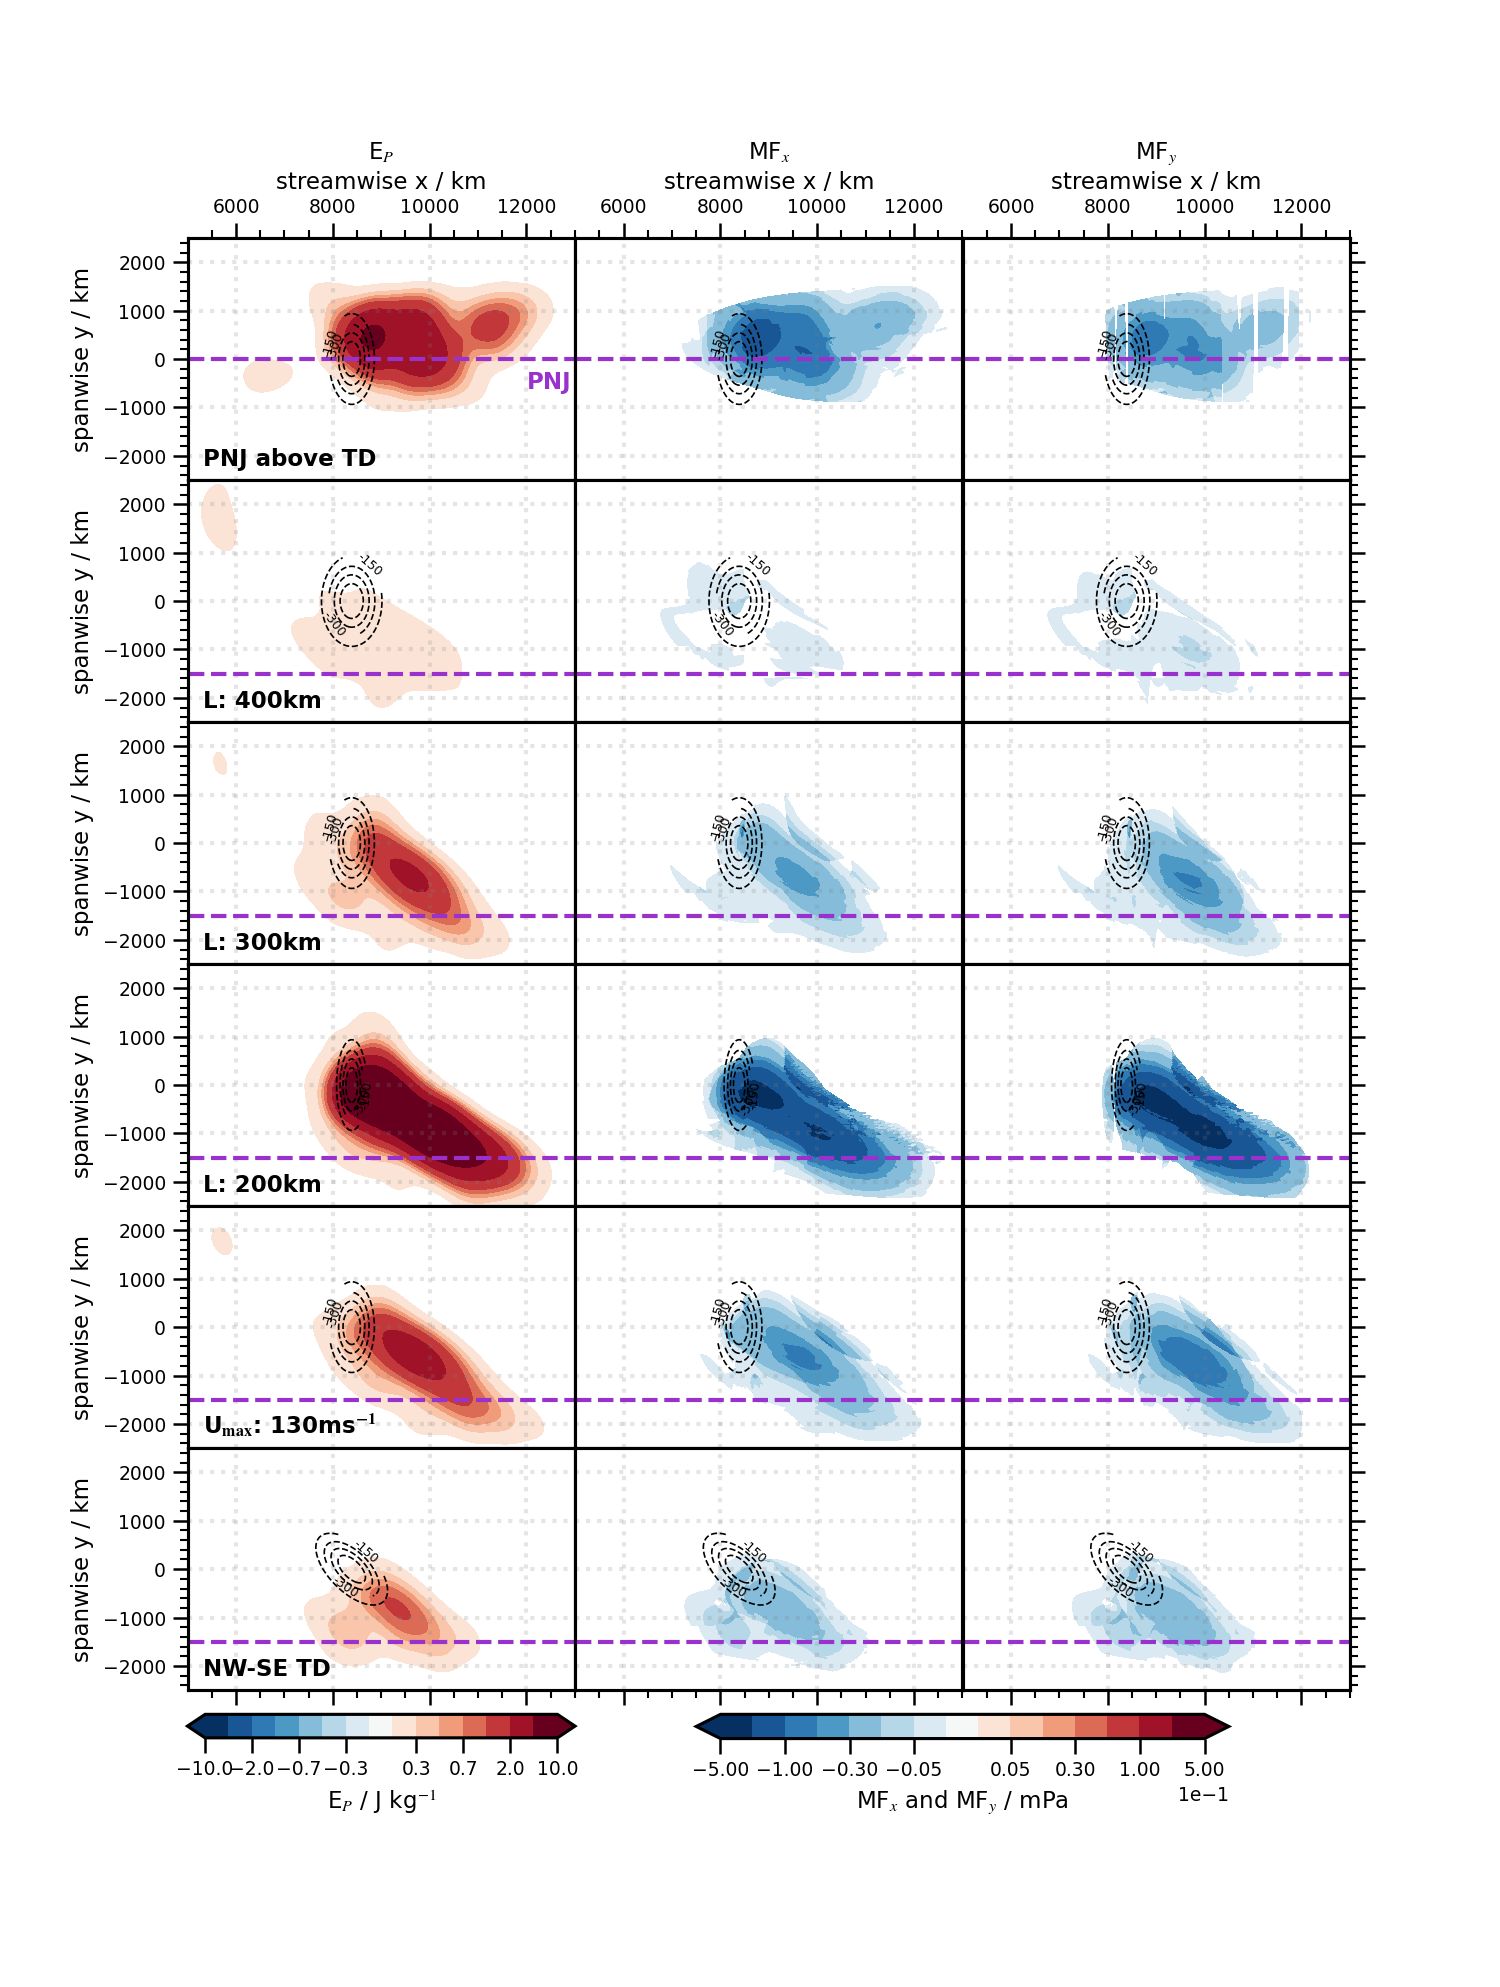
\includegraphics[width=0.99\textwidth]{figures_3D/waveletAna_fluxes_obs.png}
    \caption{Horizontal cross sections at 40km above the tropopause for five simulations with horizontal and meridional shear in a barotropic environment. Shown are $\theta$', $\lambda_x$ and $\lambda_y$ at 72h into the simulation. Dominant zonal and meridional wavelengths for each grid point are determined from wavelet analysis.}
    \label{fig:waveletAna_dudy}
\end{figure*} 